\chapter{Green Function Databases}\label{cha:gf-databases}

A Green function database stores the wavefield from a set of stations so that
seismograms for many different sources can be computed later, without running
the solver again. This is useful when you need seismograms for thousands of
trial sources at the same few stations, for example in a source inversion or
when you sample a posterior distribution with a Markov chain Monte Carlo method.
Seismograms from a 3D simulation can fit the data much better than the
approximations used in routine source inversions (Figure~\ref{fig:gf-comparison}).

\begin{figure}
\centering
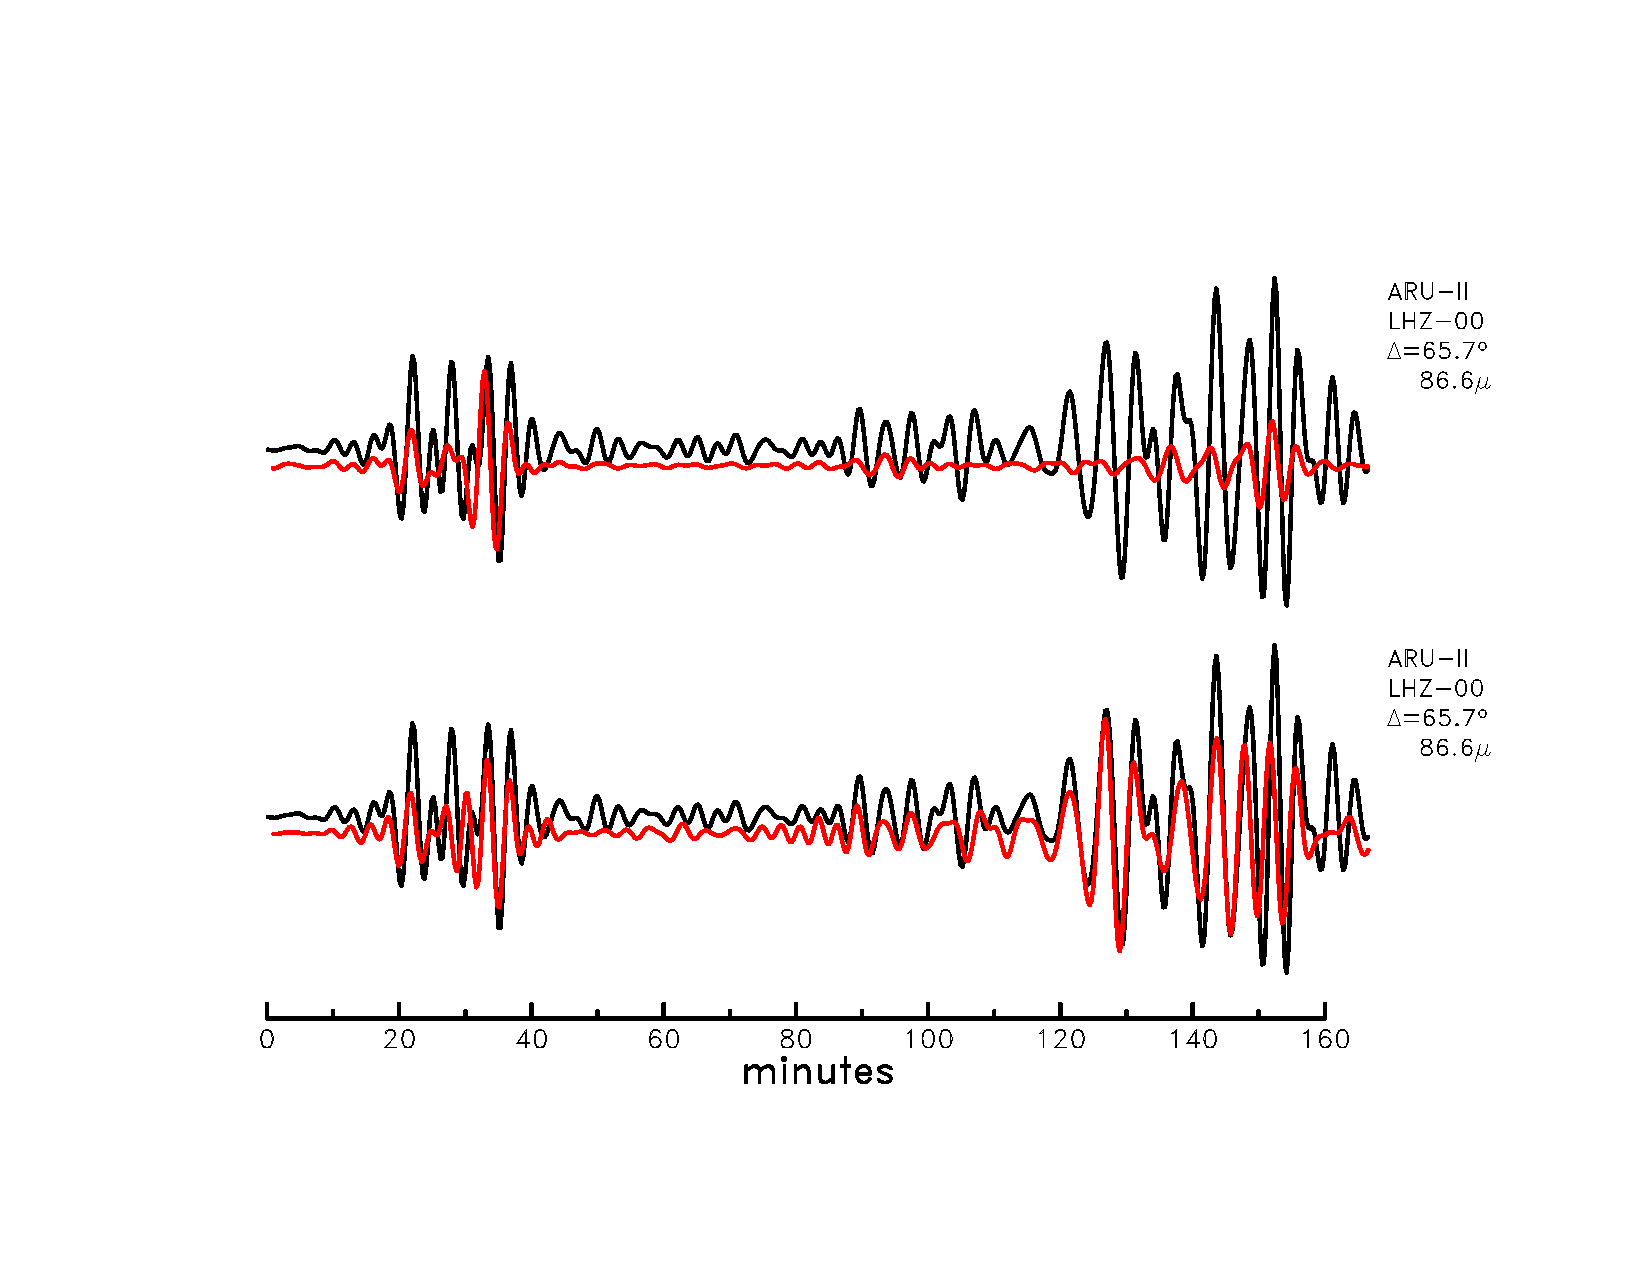
\includegraphics[width=0.6\textwidth]{figures/comparison_cropped.pdf}
\caption{\textbf{Improved fit of coupled waves.} Observed vertical-component
mantle-wave seismograms (black) for the Alaska earthquake of January 21, 2018,
and corresponding synthetic seismograms (red) recorded at Global Seismic Network
station II.ARU, Arti, Russia. In the top pair, the synthetics were calculated
using the path-average approximation, as in the GCMT analysis. In the bottom
pair, the synthetics were calculated using SPECFEM3D\_GLOBE. The main
difference is the incorporation of rotation (Coriolis effect) in the latter.
From \citet{Sawade2024}.}
\label{fig:gf-comparison}
\end{figure}

The database uses source--receiver reciprocity (Figure~\ref{fig:gf-reciprocity}).
Instead of one simulation per
earthquake, you run three simulations per station: one with a point force at
the station in the north, east and vertical direction. Each simulation stores the
displacement on a small set of spectral elements around the source locations
you expect, subsampled in time. This is the sparse reciprocal database of
\citet{Sawade2024}. From it, seismograms for any moment tensor (\texttt{CMTSOLUTION})
or force (\texttt{FORCESOLUTION}) source inside the stored elements take a
fraction of a second to compute. A database cannot give seismograms at stations
that were not simulated, or for a source outside the stored elements.

The method is not new. \citet{Zhao2006} described strain Green's tensors
computed with reciprocity and used them for source and structure studies.
\citet{Ding2021} computed a strain Green's function database with SPECFEM for
regional source inversions. \citet{Simute2022} used a regional database for
Bayesian source inversions with a 3D model of the Japanese Islands.
\citet{Sawade2024} applied the method to the whole globe, and stored only the
elements near earthquake locations.

\begin{figure}
\centering
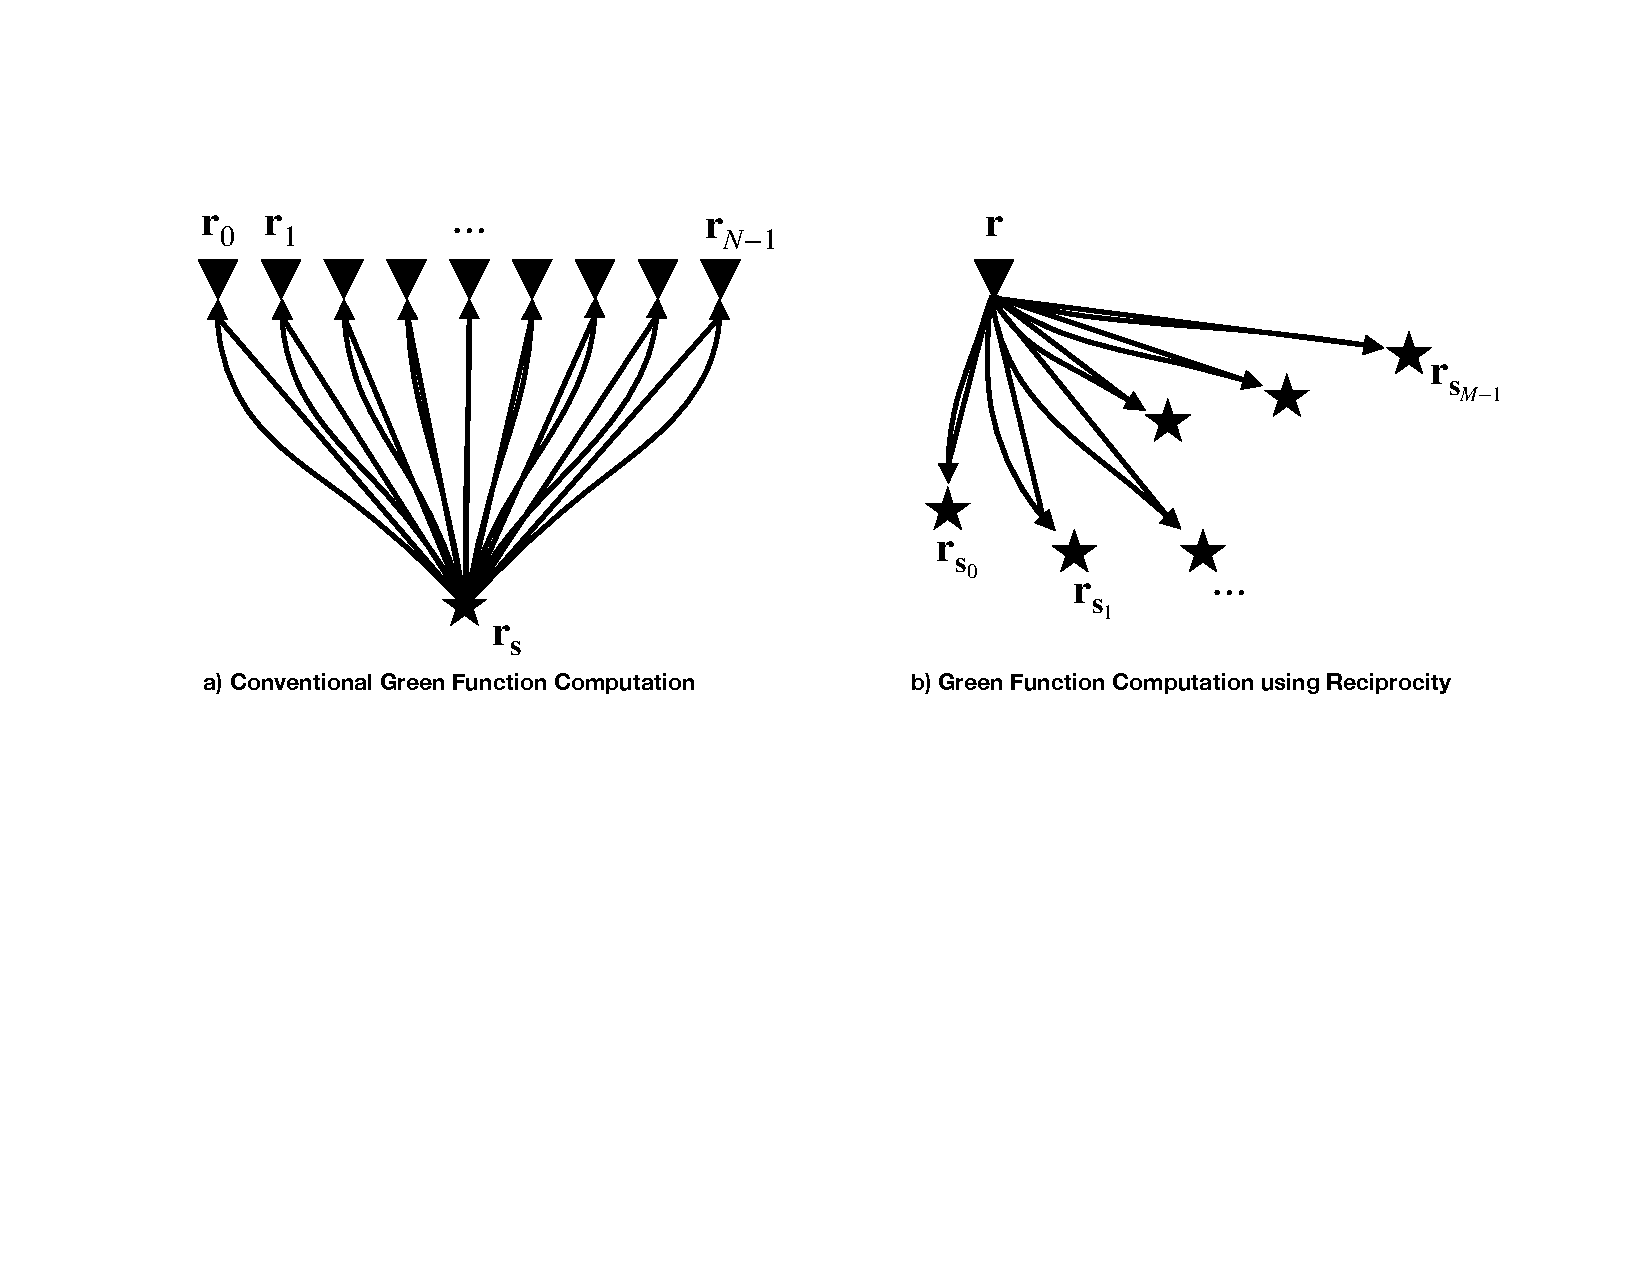
\includegraphics[width=0.9\textwidth]{figures/reg_vs_sgt.pdf}
\caption{(a) A conventional simulation has one source and gives seismograms at
all receivers. (b) With reciprocity, a simulation has a force at one receiver
and gives seismograms for all source locations. From \citet{Sawade2024}.}
\label{fig:gf-reciprocity}
\end{figure}

\paragraph{The contraction.}
By reciprocity, the displacement at station $\mathbf{x}_r$ in direction $a$
(N, E or Z) due to a moment tensor $\mathbf{M}$ at $\mathbf{x}_s$ is
\begin{equation}
u_a(\mathbf{x}_r,t) = \sum_{p,q} M_{pq}\,\epsilon^{a}_{pq}(\mathbf{x}_s,t),
\label{eq:gf-classic}
\end{equation}
where $\epsilon^{a}$ is the strain at the source due to a unit force at the
station in direction $a$. We leave out the source time function here; see
Section~\ref{sec:gf-extract}. Inside a spectral element, the strain follows from
the stored displacement $u^a_p(ijk,t)$ at the $5\times5\times5$ GLL points and the
derivatives of the Lagrange polynomials
$\ell_{ijk}(\mathbf{x}) = \ell_i(\xi)\,\ell_j(\eta)\,\ell_k(\gamma)$, where
$\xi$, $\eta$, $\gamma$ are the local coordinates of $\mathbf{x}$ in the element:
\begin{equation}
\epsilon^{a}_{pq}(\mathbf{x}_s,t) = \frac{1}{2}\sum_{i,j,k}
\left[u^a_p(ijk,t)\,\partial_q\ell_{ijk}(\mathbf{x}_s) + u^a_q(ijk,t)\,\partial_p\ell_{ijk}(\mathbf{x}_s)\right].
\end{equation}
Because $\mathbf{M}$ is symmetric and all operations are linear, we can change
the order of the sums and write Equation~(\ref{eq:gf-classic}) as
\begin{equation}
u_a(\mathbf{x}_r,t) = \sum_{p}\sum_{i,j,k} w_{p,ijk}\,u^a_p(ijk,t),
\qquad
w_{p,ijk} = \sum_q M_{pq}\,\partial_q\ell_{ijk}(\mathbf{x}_s).
\label{eq:gf-weights}
\end{equation}
The weights $w$ (375 numbers) depend only on the source, so they are computed
once. The seismogram is then one dot product per time sample, over data that
lie next to each other in memory. This is much faster than computing the strain
at every time step. For a force $\mathbf{f}$, the weights are
$w_{p,ijk} = f_p\,\ell_{ijk}(\mathbf{x}_s)$. The partial derivatives with respect
to the moment tensor and the source location use the same sum, with one weight
vector per parameter.


\section{Generating a Database}\label{sec:gf-generate}

The database is written by the solver \texttt{xspecfem3D}. The code must be
configured with HDF5, for example:
\begin{verbatim}
./configure --with-hdf5 HDF5_INC=<dir> HDF5_LIBS=-L<dir>
\end{verbatim}

\subsection{Parameters in the \texttt{Par\_file}}

The following entries control the database. They are not in the default
\texttt{DATA/Par\_file}; if they are missing, the default values are used.
\begin{description}
\item[\texttt{GF\_DATABASE\_ENABLED}] Set to \texttt{.true.} to write a database.
  Default: \texttt{.false.}
\item[\texttt{GF\_DATABASE\_PATH}] The directory of the database. All simulations
  for all stations must write to the same directory.
  Default: \texttt{OUTPUT\_FILES/gf\_database/}.
\item[\texttt{GF\_SUBSAMPLE\_STEP}] Store every $N$-th time step. The value
  \texttt{0} means automatic: about 20 samples per shortest resolved period.
  Default: \texttt{0}.
\item[\texttt{GF\_BUFFER\_SIZE}] Number of time samples kept in memory before
  they are written to disk. Default: \texttt{100}.
\item[\texttt{GF\_NEIGHBOR\_SHELLS}] Number of layers of neighbor elements
  stored around each element that contains a source location. Default: \texttt{1}.
\item[\texttt{GF\_OVERWRITE}] Write elements again even if they are already
  complete. Default: \texttt{.false.}
\end{description}
The examples (Section~\ref{sec:gf-examples}) use:
\begin{verbatim}
HDF5_ENABLED                    = .true.
USE_FORCE_POINT_SOURCE          = .true.
GF_DATABASE_ENABLED             = .true.
GF_DATABASE_PATH                = ./GFDB/
GF_SUBSAMPLE_STEP               = 0
GF_BUFFER_SIZE                  = 100
GF_NEIGHBOR_SHELLS              = 1
\end{verbatim}
Each database simulation must be a forward simulation
(\texttt{SIMULATION\_TYPE = 1}) with exactly one force with one non-zero
direction, and \texttt{USE\_FORCE\_POINT\_SOURCE = .true.} If \texttt{ROTATION} is on, the solver reverses the
rotation of the Earth for you, as reciprocity requires.

\subsection{Input files}

\texttt{DATA/GF\_LOCATIONS} lists the source locations the database must cover,
one per line as latitude, longitude (degrees) and depth (km). Lines that start
with \texttt{\#} are comments:
\begin{verbatim}
# latitude  longitude  depth_km
-35.909   -72.733   35.0
-5.812    -75.270   122.6
\end{verbatim}
The solver finds the element that contains each location and adds
\texttt{GF\_NEIGHBOR\_SHELLS} layers of neighbor elements.
Figure~\ref{fig:subselection} shows the elements selected for all
earthquakes in the GCMT catalog.

\begin{figure}
    \centering
    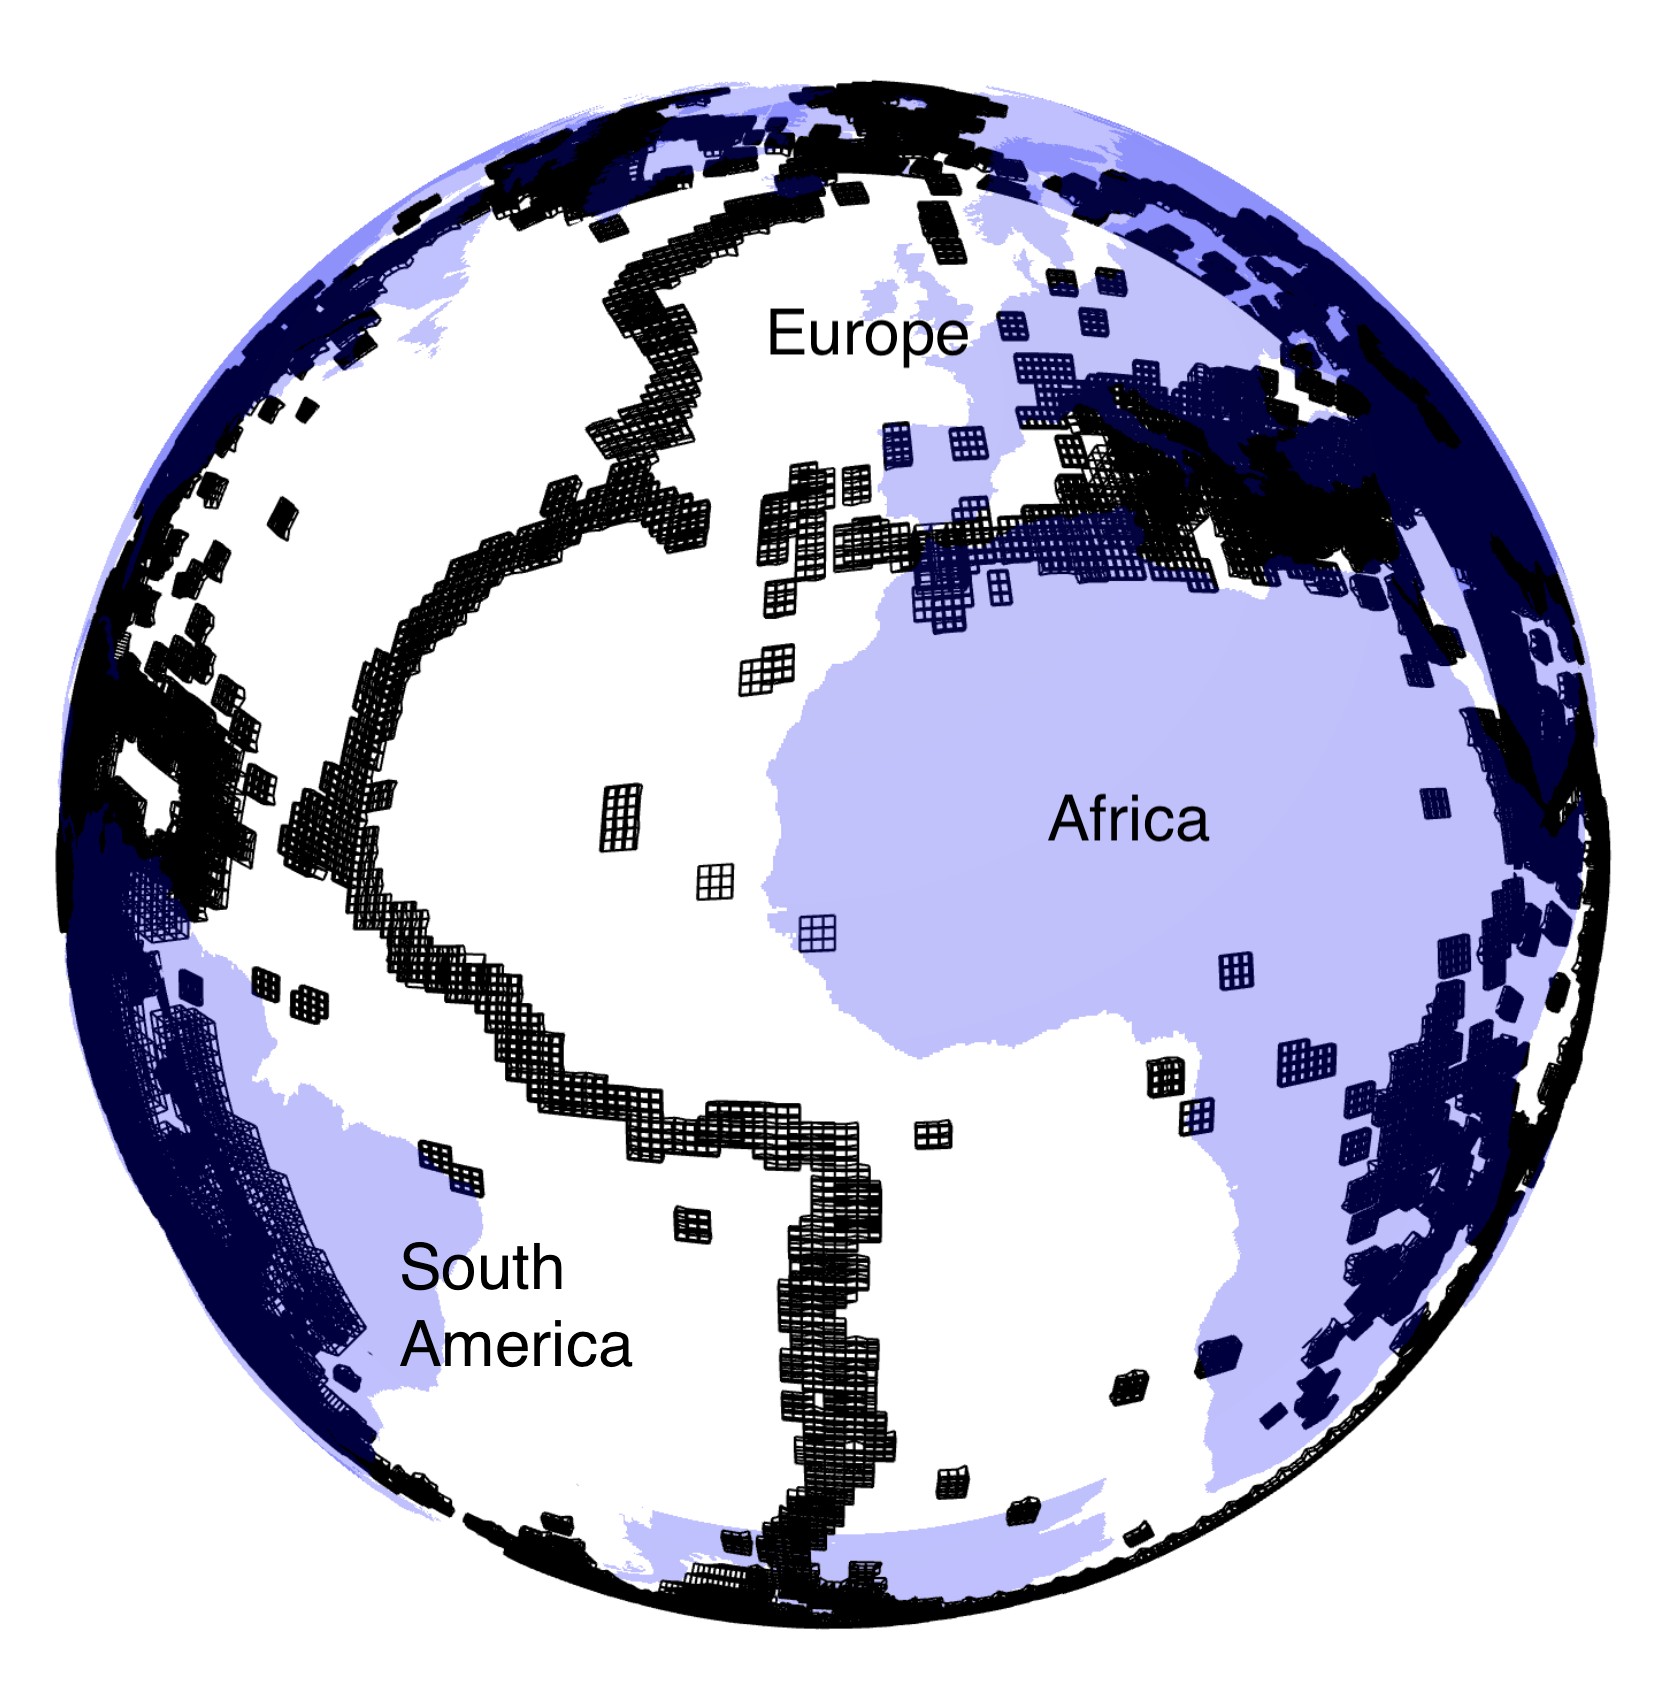
\includegraphics[width=0.3\textwidth, trim={0.4in 0.5in 0.4in 0.5in}, clip]{figures/globenew_annotated.png}
    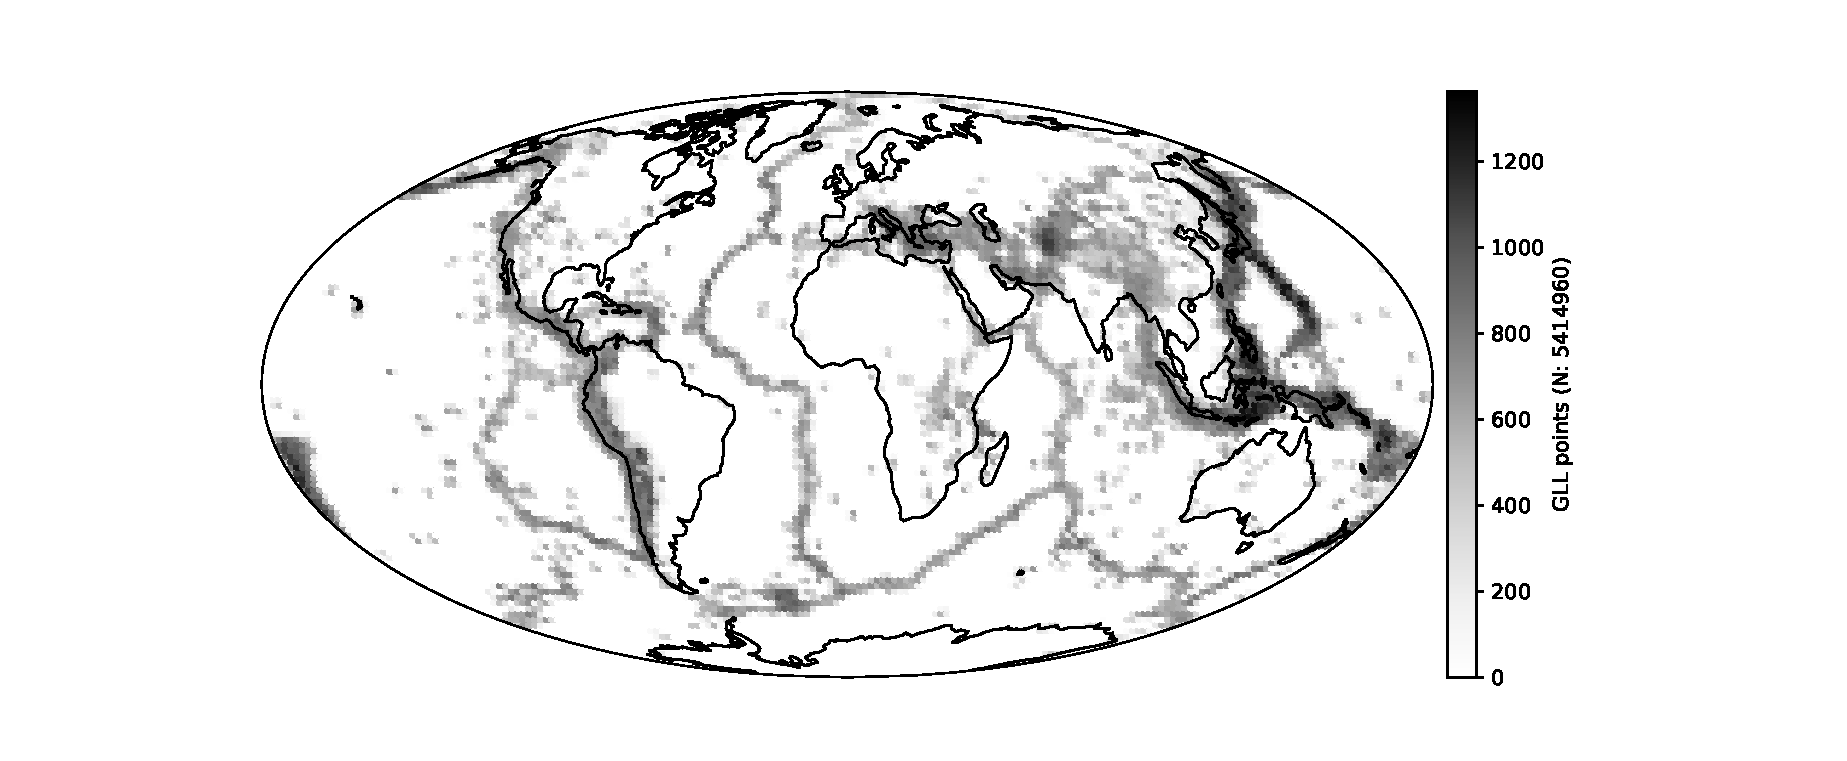
\includegraphics[width=0.68\textwidth, trim={1.5in 0.4in 1.5in 0.25in}, clip]{figures/numberofgllpoints.pdf}
    \caption{\textbf{Subselected elements of a global mesh} -- \textit{Left}: View of subselected spectral-element edges in a 3-D Earth. The full GCMT catalogue \citep{ekstrom2012global} provides the seismicity for subselection. Some isolated areas show that the tagged and neighbouring elements are considered.
    We plotted the continents at the surface at radius $R_c = 1.05\cdot 6371~\mathrm{km}$ in transparent, light blue and a white sphere at $R_s = 6371~\mathrm{km} - 800~\mathrm{km}$ for clarity.
    \textit{Right}: Hexagonal histogram of GLL points. The colour indicates the number of points in each hexagon, and the total number of GLL points (5,414,960) is shown in the colour-bar label. The histogram shows how subduction zones produce a higher density of GLL points due to the vertical extent of seismicity. In contrast, mid-ocean ridges show smaller numbers of GLL points per bin.
    From \citet{Sawade2024}.}
    \label{fig:subselection}
\end{figure}

\texttt{DATA/FORCESOLUTION} puts a force at the station. You need three simulations
per station, one for each direction. The depth is the burial of the station in
\textbf{km} (the \texttt{STATIONS} file gives the burial in m). The first line
must give the station as \texttt{NET.STA}. For station IU.RCBR in the north direction:
\begin{verbatim}
FORCE  IU.RCBR
time shift:     0.0000
f0:             0.0500
latitude:      -5.8274
longitude:     -35.9014
depth:         0.1090
source time function: 0
factor force source:  1.0d15
comp dir vect source E:   0.0
comp dir vect source N:   1.0
comp dir vect source Z:   0.0
\end{verbatim}
All simulations must use the same mesh. Simulations for different stations can
run at the same time. When all simulations are done, the script
\url{utils/green_function/gf_build_manifest.py} writes an index of the
elements. The index is optional, but it makes opening the database faster.

\subsection{Source time function of the database}

The solver ignores the half duration in the \texttt{FORCESOLUTION}. It uses
its own Gaussian source time function with half duration
$h_{\mathrm{db}} = T_{\mathrm{min}}/10$, where $T_{\mathrm{min}}$ is the
shortest period the mesh resolves. The Gaussian is low-pass filtered at the
Nyquist frequency of the stored samples, so that the subsampling does not
alias. It is written to \texttt{OUTPUT\_FILES/gf\_stf.txt}. At extraction,
this source time function is replaced by the one of your source
(Section~\ref{sec:gf-extract}).

\subsection{Output}

The database is a directory of HDF5 files:
\begin{verbatim}
GFDB/mesh_info.h5                    time axis, mesh flags, topography
GFDB/stations/NET.STA.h5             station and source time function
GFDB/elements/<id>/coordinates.h5    GLL point coordinates of one element
GFDB/elements/<id>/NET.STA.h5        displacement of one element, one station
\end{verbatim}
The database stores \emph{displacement}, not strain. Each element file holds
an array of shape $3\times3\times5\times5\times5\times n_t$ (force direction,
displacement component, GLL points, time samples) in single precision, so one
element and one station need $3\cdot3\cdot125\cdot n_t\cdot4$ bytes.


\section{Extracting Seismograms}\label{sec:gf-extract}

The extraction library is in \texttt{src/gf3d/}. Build it with
\begin{verbatim}
make gf3d
\end{verbatim}
This creates the command line tool \texttt{bin/xgf3d}, the libraries
\texttt{lib/libgf3d.a} and \texttt{lib/libgf3d.so}, and the interface files
\texttt{include/gf3d.mod} (Fortran) and \texttt{include/gf3d.h} (C). There are
three ways to use the library: the command line tool, Fortran, and Python. All three
use the same code and give the same numbers.

Each extraction locates the source in the database, builds the weights of
Equation~(\ref{eq:gf-weights}), computes the trace at each station, and
applies the source time function. Seismograms are in meters [m], with
components N, E and Z. Time is in seconds [s], with $t=0$ at the centroid time
(origin time plus \texttt{time shift}). By default, the output starts $1.5$
half durations before the centroid time, as in a forward simulation of the solver.

\paragraph{Source time function.}
The stored traces already contain the database Gaussian of half duration
$h_{\mathrm{db}}$. A forward simulation with a \texttt{CMTSOLUTION} uses an error
function of half duration $h = h_{\mathrm{CMT}}/1.628$
(see Figure~\ref{fig:gauss.vs.triangle}). The convolution of two Gaussians is
a Gaussian whose squared half duration is the sum of the two squared half
durations. Therefore, the code convolves the trace once, with an error function
of half duration
\begin{equation}
h_{\mathrm{corr}} = \sqrt{h^2 - h_{\mathrm{db}}^2},
\end{equation}
and the result matches a forward simulation with half duration $h$
\citep{Sawade2024}. Force sources are treated in the same way. If
$h \le h_{\mathrm{db}}$, no correction is possible: the output keeps the
half duration of the database, and the header of the output reports
\texttt{GUARD}. In the global example, $h_{\mathrm{db}} = 6.9$~s.

\paragraph{Element cache.}
For each source, the library reads the displacement of one element for all
stations from disk. For a large database, this read takes most of the time.
If you compute many sources that are close to each other, for example in a
Markov chain Monte Carlo loop, open the database with
\texttt{max\_elements = N}. The library then keeps the $N$ most recently used
elements in memory. When the cache is full, it removes the element that was
used least recently. The results are the same as without the cache. Each
element needs $9\cdot125\cdot n_t\cdot n_{\mathrm{sta}}\cdot4$ bytes of memory.
The default is \texttt{0}, which means no cache. If the code is configured with
\texttt{-{}-enable-openmp}, an extraction from the cache computes the stations in
parallel. As an example, for 185 stations and 3725 time samples, one extraction takes
about 2.2~s from disk, 0.5~s from the cache on one core, and 0.02~s from the
cache on 32 threads.

\subsection{Command line tool}

\texttt{xgf3d} reads a database and a source file, and writes seismograms.
It detects from the file content whether the source is a \texttt{CMTSOLUTION}
or a \texttt{FORCESOLUTION}. The main modes are:
\begin{verbatim}
xgf3d --info <GFDB>                                describe a database
xgf3d --locate <GFDB> <lat> <lon> <depth_km>       locate a position
xgf3d --seis <GFDB> <SOURCE> <outdir> [options]    compute seismograms
\end{verbatim}
For example:
\begin{verbatim}
mkdir -p OUTPUT_GF
bin/xgf3d --seis GFDB DATA/CMTSOLUTION OUTPUT_GF
\end{verbatim}
This writes binary SAC files \texttt{NET.STA.BXN.sem.sac} (and \texttt{BXE},
\texttt{BXZ}) for every station in the database. The output directory must exist.
Useful options are:
\begin{itemize}
\item \texttt{-{}-format}: \texttt{sac} (default), \texttt{sacan}, \texttt{ascii} or \texttt{all},
\item \texttt{-{}-partials 1}: also write the partial derivatives with respect to
  the six moment tensor components,
\item \texttt{-{}-partials 2}: also add latitude, longitude, depth and centroid time.
\end{itemize}
See \texttt{xgf3d -{}-help} for all options.

\subsection{Fortran API}

The Fortran module \texttt{gf3d} gives the same functions to your own program.
Every routine returns an error code \texttt{ierr}; the library never stops
your program. A minimal program:
\begin{verbatim}
program extract
  use gf3d
  implicit none
  type(t_gfdb) :: db
  type(t_gf_source) :: src
  double precision, allocatable :: synt(:,:,:), t(:)
  double precision :: t0
  integer :: ierr

  call gf_open('GFDB', db, ierr, max_elements = 4)
  call check(ierr)
  call gf_read_cmt_source(db, 'CMTSOLUTION', src, ierr)
  call check(ierr)
  call gf_default_t0(src, t0, ierr)    ! start time of a forward simulation
  call check(ierr)
  call get_seismograms(db, src, t0, synt, ierr, t)
  call check(ierr)

  ! synt(station, component N/E/Z, time) in m; t(time) in s
  print *, db%stations(1)%id, maxval(abs(synt(1,:,:)))
  call gf_release(db)

contains

  subroutine check(ierr)
    integer, intent(in) :: ierr
    if (ierr /= GF_OK) then
      print *, trim(gf_errmsg)
      stop 1
    endif
  end subroutine check

end program extract
\end{verbatim}
Compile it with the same compiler that built the library:
\begin{verbatim}
gfortran extract.f90 -I<specfem>/include -L<specfem>/lib -lgf3d \
         -Wl,-rpath,<specfem>/lib
\end{verbatim}
\texttt{get\_partials} returns the partial derivatives as well. A complete
example is in
\url{EXAMPLES/green_function_database/global/api_demos/fortran/}.

\subsection{Python API}

The Python package \texttt{gf3d} calls \texttt{lib/libgf3d.so}. Install it with
\begin{verbatim}
pip install -e utils/green_function
\end{verbatim}
A minimal script:
\begin{verbatim}
import gf3d

with gf3d.Database("GFDB", max_elements=4) as db:
    cmt = gf3d.CMTSource.read("CMTSOLUTION")
    r = db.seismograms(cmt)

print(r.station_ids)   # ['II.RPN', 'IU.RCBR', 'IU.SJG', 'IU.TRQA']
print(r.data.shape)    # (stations, 3, time): components N, E, Z in m
print(r.t[:3])         # time in s, t = 0 at the centroid time
\end{verbatim}
\texttt{db.partials(cmt)} also returns the partial derivatives in
\texttt{r.dp}, and \texttt{r.to\_stream()} converts the result to an ObsPy
\texttt{Stream}. Errors raise a \texttt{gf3d.GF3DError}. See
\url{utils/green_function/gf3d/README.md} and
\url{EXAMPLES/green_function_database/global/api_demos/python/} for more.

\subsection{Element data and weights}\label{sec:gf-weights-api}

A sampler, for example Markov chain Monte Carlo or Hamiltonian Monte Carlo,
evaluates many sources in the same element. It can be faster to do the sum of
Equation~(\ref{eq:gf-weights}) yourself, on a GPU for example, and call the
library only for the two ingredients:
\begin{itemize}
\item \texttt{element\_block}: the stored displacement of one element for a set
  of stations, in the order the sum reads it. It is read once per element.
\item \texttt{weights}: the weights $w$ of a source, the weights of its partial
  derivatives, and an amplitude factor per station. It is called once per
  source and reads no displacement.
\end{itemize}
For station $s$, force component $a$ and stored sample $t$, the trace before
the source time function is
\begin{equation}
x_{s,a}(t) = \mathrm{scale}_s \sum_{m} u_{s,a}(t,m)\, w_m,
\qquad m = p + 3\,(i + 5j + 25k),
\end{equation}
and a partial derivative is the same sum with its own weights. In Python:
\begin{verbatim}
import numpy as np
import gf3d

db = gf3d.Database("GFDB")
cmt = gf3d.CMTSource.read("CMTSOLUTION")

W = db.weights(cmt, kind=2)                # W.w (375,), W.dw (9, 375), W.scale
u = db.element_block(W.location.ielem)     # (stations, 3, time, 375), float32
x = W.scale[:, None, None] * (u @ W.w)     # (stations, 3, time)
\end{verbatim}
The result $x$ does not contain the source time function yet. This is on
purpose: you choose the source time function. \texttt{gf3d.stf\_kernel(kind,
hdur, dt, trunc)} returns the kernel the library uses, and \texttt{db.plan(cmt)}
gives the values the library would use for this source. The header file
\texttt{include/gf3d.h} gives the exact formula of the convolution. With the
library's own kernel, the result is \texttt{db.seismograms(cmt)} up to
rounding. The time derivative has no weight: a change of the centroid time is
a shift of the trace.

\texttt{element\_block(ielem, nt=n)} reads only the first $n$ samples. The
source time function at the last \texttt{plan.khalf} samples needs data after
them, so read that many more samples than you keep. One element needs
$n_{\mathrm{sta}}\cdot 3\cdot n\cdot 375\cdot 4$ bytes; for 142 stations and
917 samples that is 0.59~GB, read in about 0.4~s. A call of \texttt{weights}
takes less than 0.1~ms. The function \texttt{element\_block} does not use the
element cache. The same calls exist in C (\texttt{gf3d\_element\_block},
\texttt{gf3d\_weights}, \texttt{gf3d\_stf\_kernel}) and in Fortran
(\texttt{gf\_element\_export}, \texttt{gf\_source\_weights},
\texttt{gf\_stf\_taps}). A complete example is
\url{EXAMPLES/green_function_database/global/api_demos/python/gf3d_sampler_demo.py}.


\section{Examples}\label{sec:gf-examples}

There are two examples in \texttt{EXAMPLES/green\_function\_database/}: a global
one (6 chunks, 4 stations) and a regional one (1 chunk, 3 stations). Both use the
same Snakemake workflow, so we only describe the global example. Each
example builds a database, runs forward simulations of the same sources with
the solver, and compares the two.

\subsection{Global example}

\begin{enumerate}
\item Configure and build the code with HDF5, then build the solver and the
  library (\texttt{make all} and \texttt{make gf3d}).

\item Install the Python packages of the workflow:
\begin{verbatim}
cd EXAMPLES/green_function_database
uv sync
\end{verbatim}

\item Run the workflow:
\begin{verbatim}
cd global
snakemake -j1
\end{verbatim}
It runs 24 MPI processes per simulation by default. To change this, use
\begin{verbatim}
snakemake -j1 --config NPROC=<n>
\end{verbatim}
The workflow does the following steps:
\begin{itemize}
\item run the mesher once in \texttt{db\_base/},
\item run three simulations per station (N, E, Z), all writing to \texttt{GFDB/},
\item build the element index of the database,
\item run two forward simulations with the solver, one for each source in
  \texttt{validation\_data/} (a CMT source and a force source),
\item compute the same two sources from the database with
  \texttt{xgf3d -{}-seis},
\item compare the seismograms.
\end{itemize}
On a node with two GPUs, the full workflow takes about 40 minutes.

\item Look at the results in \texttt{validation\_output/}. It contains a figure
  per station, a record section per source type, and a summary table
  \texttt{gf\_compare\_summary.md}. The workflow fails if the relative L2 misfit
  between the database and the forward seismograms is larger than
  $5\cdot10^{-3}$ at any station. In the global example, the largest misfit is
  about $2.5\cdot10^{-3}$.
\end{enumerate}

If you change \texttt{GF\_SUBSAMPLE\_STEP} or the stations, delete the old
database and simulations first:
\begin{verbatim}
snakemake clean_database clean_simulations
\end{verbatim}
